% https://en.wikipedia.org/wiki/File:DIT-FFT-butterfly.svg

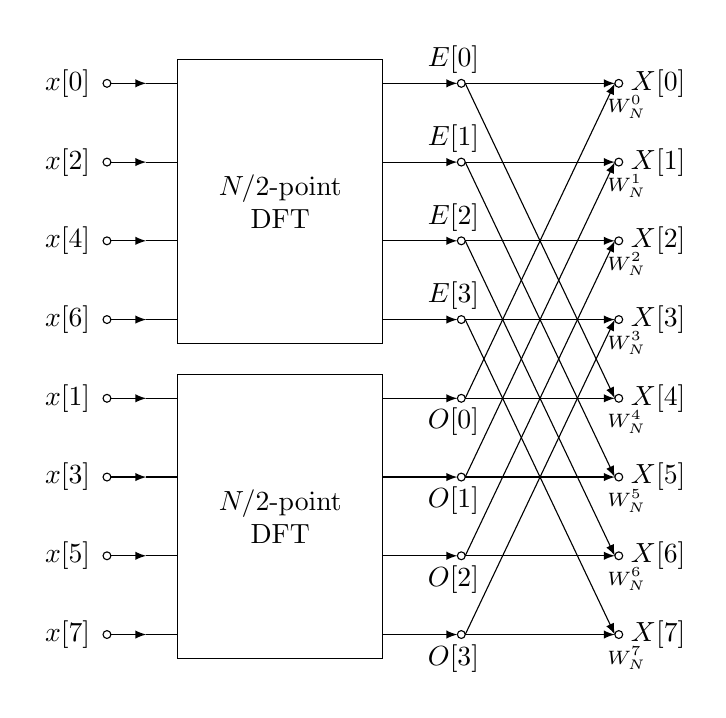
\begin{tikzpicture}% Example:
  \draw[fill=white, draw=white] (-0.5, 0.7) rectangle (8, -7.7); 
  \draw (0,0) node {$x[0]$};
  \draw (0,-1) node {$x[2]$} ;
  \draw (0,-2) node {$x[4]$} ;
  \draw (0,-3) node {$x[6]$} ;

  \draw (0,-4) node {$x[1]$} ;
  \draw (0,-5) node {$x[3]$} ;
  \draw (0,-6) node {$x[5]$} ;
  \draw (0,-7) node {$x[7]$} ;

  % arrow on the right of x's
  \foreach \n in {0,...,7} {
    \draw (0.5,-\n) circle(0.05)[fill=white]; 
    \draw [-latex] (0.55,-\n) -- (1, -\n); 
    \draw (1, -\n) -- (1.4, -\n); 
  }

  % blocks
  \draw(1.4, 0.3) rectangle (4, -3.3); 
  \draw(1.4, -3.7) rectangle (4, -7.3); 
  \draw(2.7, -1.5) node[text centered, text width=2cm] {$N/2$-point DFT};
  \draw(2.7, -5.5) node[text centered, text width=2cm] {$N/2$-point DFT};

  % E's and O's 
  \foreach \n in {0,...,7} {
    \draw [-latex] (4,-\n) -- (4.95, -\n); 
    \draw (5,-\n) circle(0.05)[fill=white]; 
  }
  \foreach \n in {0,...,3} {
    \draw (4.9,-\n + 0.3) node {$E[\n]$};
  }
  \foreach \n in {0,...,3} {
    \draw (4.9,-\n - 4 - 0.3) node {$O[\n]$};
  }

  % X's 
  \foreach \n in {0,...,7} {
    \draw (7,-\n) circle(0.05)[fill=white]; 
    \draw (7.5,-\n) node {$X[\n]$};
  }

  % Connecting X and E
  \foreach \n in {0,...,7} {
    \draw [-latex] (5.05, -\n) -- (6.95, -\n);
  }
  \foreach \n in {0,...,3} {
    \draw [-latex] (5.05, -\n) -- (6.95, -\n - 4);
  }
  \foreach \n in {0,...,3} {
    \draw [-latex] (5.05, -\n-4) -- (6.95, -\n);
  }

  % W's
  \foreach \n in {0,...,7} {
    \draw (7.1,-\n - 0.3) node {\scriptsize $W_N^{\n}$};
  }
\end{tikzpicture}
